\documentclass[titlepage]{jarticle}
\usepackage{h31ec-exp}
\usepackage[dvipdfmx]{graphicx}
\usepackage{here}
\usepackage{multirow}

\title{電気抵抗の測定と接続}
\grade{1年39番}%
\author{鷲尾 優作}
\team{}
\date{令和2年2月28日}
\expdate{令和2年2月25日}
\coauthor{%
  --番 & -- --\\
  --番 & -- --\\
  --番 & -- --}

\begin{document}
\maketitle

\section{本実験の目的}
\begin{itemize}
    \item 未知抵抗の測定を通して,ホイートストンブリッジの原理と使用方法を学ぶ
\end{itemize}

\section{理論}
図1の回路において,抵抗値$A$,$B$,$R$を調整し\\
検流計$G$の電流をゼロにするとブリッジが平衡状態となり式(1)が成立する.\\
また変形し式(2)が成り立つ。\\
\begin{figure}[H]
    \begin{center}
        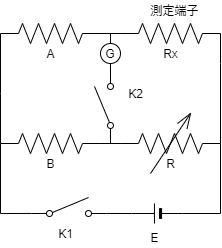
\includegraphics[width=5cm]{image/image01.png}
        \caption{ホイートストンブリッジ原理図}
    \end{center}
\end{figure}
\begin{equation}
    A×R = B×R_x
\end{equation}
\begin{equation}
    R_x = A/B×R
\end{equation}
式(2)より$A$,$B$,$R$が決まると$R_x$の値が求まる.$A/B$を倍率(比例辺),$R$を測定辺(加減辺)という.\\
今回使用するホイートストンブリッジは,倍率ダイヤル,測定辺ダイヤル,検流計スイッチ,測定用電源,測定用端子が\\
ひとつの箱におさめられている.
\section{実験内容}
ホイートストンブリッジを使用し,3つの未知抵抗器$R1$,$R2$,$R3$の直列,並列,並直列\\
それぞれの接続パターンの合成抵抗値を測定,誤差率の計算を行いまとめる.\\
倍率ダイヤルの設定値は表1の理論値を参考に選択する.

\section{使用器具}
\begin{enumerate}
    \item ホイートストンブリッジ\\用途 抵抗値測定のため\\商品名YOKOGAWA Type 2755
    \item RLCボックス\\用途 実験用未知抵抗\\商品名不明
    \item 接続コード\\用途 ホイートストンブリッジとRLCボックスの接続のため\\商品名不明
\end{enumerate}

\section{実験結果}

% Please add the following required packages to your document preamble:
% \usepackage{multirow}
\begin{table}[H]
    \begin{tabular}{l|l|l|l|l|l|l}
        \hline\hline
        \multirow{2}{*}{番号} & \multicolumn{1}{c|}{\multirow{2}{*}{接続方法}} & \multicolumn{3}{l|}{実測値} & \multirow{2}{*}{理論値{[}Ω{]}} & \multirow{2}{*}{誤差率{[}\%{]}} \\ \cline{3-5}
         & \multicolumn{1}{c|}{} & 測定辺 & 倍率 & 抵抗値{[}Ω{]} &  &  \\ \hline
    \multicolumn{1}{l|}{1} & $R1$ & 0.1 & 0998 & 99.8 & \multicolumn{1}{l|}{100.0} & 0.2 \\
    \multicolumn{1}{l|}{2} & $R2$ & 0.1 & 1994 & 199.4 & \multicolumn{1}{l|}{200.0} & 0.3 \\
    \multicolumn{1}{l|}{3} & $R3$ & 0.1 & 2998 & 299.8 & \multicolumn{1}{l|}{300.00} & 0.1 \\ \hline
    \multicolumn{1}{l|}{4} & $R1 + R2$ & 0.1 & 2992 & 299.2 & \multicolumn{1}{l|}{300.00} & 0.3 \\
    \multicolumn{1}{l|}{5} & $R1 + R3$ & 0.1 & 3996 & 399.6 & \multicolumn{1}{l|}{400.00} & 0.1 \\
    \multicolumn{1}{l|}{6} & $R2 + R3$ & 0.1 & 4996 & 499.6 & \multicolumn{1}{l|}{500.00} & 0.1 \\
    \multicolumn{1}{l|}{7} & $R1 + R2 + R3$ & 0.1 & 5996 & 599.6 & \multicolumn{1}{l|}{600.00} & 0.1 \\
    \multicolumn{1}{l|}{8} & $R1 // R2$ & 0.1 & 0665 & 66.5 & \multicolumn{1}{l|}{66.67} & 0.3 \\
    \multicolumn{1}{l|}{9} & $R1 // R3$ & 0.1 & 0749 & 74.9 & \multicolumn{1}{l|}{75.00} & 0.1 \\
    \multicolumn{1}{l|}{10} & $R2 // R3$ & 0.1 & 1198 & 119.8 & \multicolumn{1}{l|}{120.00} & 0.2 \\
    \multicolumn{1}{l|}{11} & $R1 // R2 // R3$ & 0.1 & 0545 & 54.5 & \multicolumn{1}{l|}{54.58} & 0.1 \\
    \multicolumn{1}{l|}{12} & $R1 + R2 // R3$ & 0.1 & 2193 & 219.3 & \multicolumn{1}{l|}{220.00} & 0.3 \\
    \multicolumn{1}{l|}{13} & $R2 + R1 // R3$ & 0.1 & 2743 & 274.3 & \multicolumn{1}{l|}{275.00} & 0.3 \\
    \multicolumn{1}{l|}{14} & $R3 + R1 // R2$ & 0.1 & 3659 & 365.9 & \multicolumn{1}{l|}{366.67} & 0.2 \\
    \multicolumn{1}{l|}{15} & $(R1 + R2) // R3$ & 0.1 & 1497 & 149.7 & \multicolumn{1}{l|}{150.00} & 0.2 \\
    \multicolumn{1}{l|}{16} & $(R1 + R3) // R2$ & 0.1 & 1330 & 133.0 & \multicolumn{1}{l|}{133.33} & 0.2 \\
    \multicolumn{1}{l|}{17} & $(R2 + R3) // R1$ & 0.1 & 0831 & 83.1 & \multicolumn{1}{l|}{83.33} & 0.3 \\ \hline
    \end{tabular}
    \end{table}

\section{課題}
\subsection{(1)}
図1の回路図から式(1)を導出せよ
\begin{eqnarray}
    検流計GのなのでGのある配線は無視できる \nonumber\\
    よってAとR_xの直列,BとRの直列同士の並列回路とみなせるので \nonumber\\
    A×R=B×R_x \nonumber
\end{eqnarray}
\subsection{(2)}
ホイートストンブリッジのように,検流計などによって電流がゼロになることを利用し,\\
物理量を測定する方法を「零位法」.電圧計,電流計などのように,針の触れ角度(偏位)によって\\
物理量を測定する方法を「偏位法」という.「零位法」が「偏位法」に比べて,原理的に測定誤差が\\
少ない理由を調査・考察して述べよ.\\

1)測定量の結果として計測する「偏位法」と比較して「零位法」は\\
平衡の検知で計測するので,測定の基準の精度と同じ精度で測定できる.\\
2)測定対象のエネルギーを奪って使い計測結果を表示する「偏位法」に対して\\
「零位法」は測定時対象は平衡しているのでほぼエネルギーを奪うことがないため\\
対象に影響を与えず高精度で測定ができる

\end{document}